\documentclass[fleqn]{article}
\oddsidemargin 0.0in
\textwidth 6.0in
\thispagestyle{empty}
\usepackage{import}
\usepackage{amsmath}
\usepackage[backend=bibtex]{biblatex}
\usepackage[utf8]{inputenc}
\usepackage{csquotes}
\usepackage{graphicx}
\usepackage{flexisym}
\usepackage{calligra}
\usepackage{amssymb}
\usepackage{bigints} 
\usepackage[english]{babel}
\usepackage{float}
\usepackage[colorinlistoftodos]{todonotes}
\usepackage{blindtext}
\usepackage{hyperref}

\addbibresource{references.bib}

\hypersetup{
  colorlinks=true,
  linkcolor=blue,
  filecolor=magenta,      
  urlcolor=cyan,
  pdfpagemode=FullScreen
}

\DeclareMathAlphabet{\mathcalligra}{T1}{calligra}{m}{n}
\DeclareFontShape{T1}{calligra}{m}{n}{<->s*[2.2]callig15}{}
\newcommand{\scriptr}{\mathcalligra{r}\,}
\newcommand{\boldscriptr}{\pmb{\mathcalligra{r}}\,}


\setlength{\arrayrulewidth}{0.5mm}
\setlength{\tabcolsep}{18pt}
\renewcommand{\arraystretch}{1.5}

\definecolor{hwColor}{HTML}{AD53BA}

\begin{document}

  \begin{titlepage}

    \newcommand{\HRule}{\rule{\linewidth}{0.5mm}}

    \center

    \begin{center}
      
\includegraphics[height=11cm, width=11cm]{asu.png}
    \end{center}

    \vline

    \textsc{\LARGE Advanced Laboratory I}\\[1.5cm]

    \HRule \\[0.5cm]
    { \huge \bfseries Pulsed NMR}\\[0.4cm] 
    \HRule \\[1.0cm]

    \textbf{Behnam Amiri}

    \bigbreak

    \textbf{Prof: Ralph Chamberlin}

    \bigbreak

    \textbf{Lab Partners: Daniel Henningsen, Micah Smith, Srihari Ravi}

    \bigbreak

    \textbf{{\large \today}\\[2cm]}

    \vfill

  \end{titlepage}

  \textbf{Abstract}

  \vspace{10px}

  This lab report represents the experimental procedure we did to learn about the \emph{Pulsed NMR} \textcite{One}

  \vspace{20px}


  \textbf{I. Introduction}

  \vspace{10px}

  TODO 

  \vspace{20px}


  \textbf{II. Background Information}

  \vspace{10px}

  TODO 

  \vspace{20px}


  \textbf{III. Theory}

  \vspace{10px}

  TODO 

  \vspace{20px}


  \textbf{IV. Experimental Procedure}

  \vspace{10px}

  We followed the given steps in the lab. TODO...
  
  \vspace{20px}

  \textbf{V. Results}

  \vspace{10px}

  The following plots are our results from this Pulsed NMR experiment. The second and third plots data are from Dr.Chamberlin due to the fact that our recorded data 
  was not correct for some reason.

  \pagebreak

  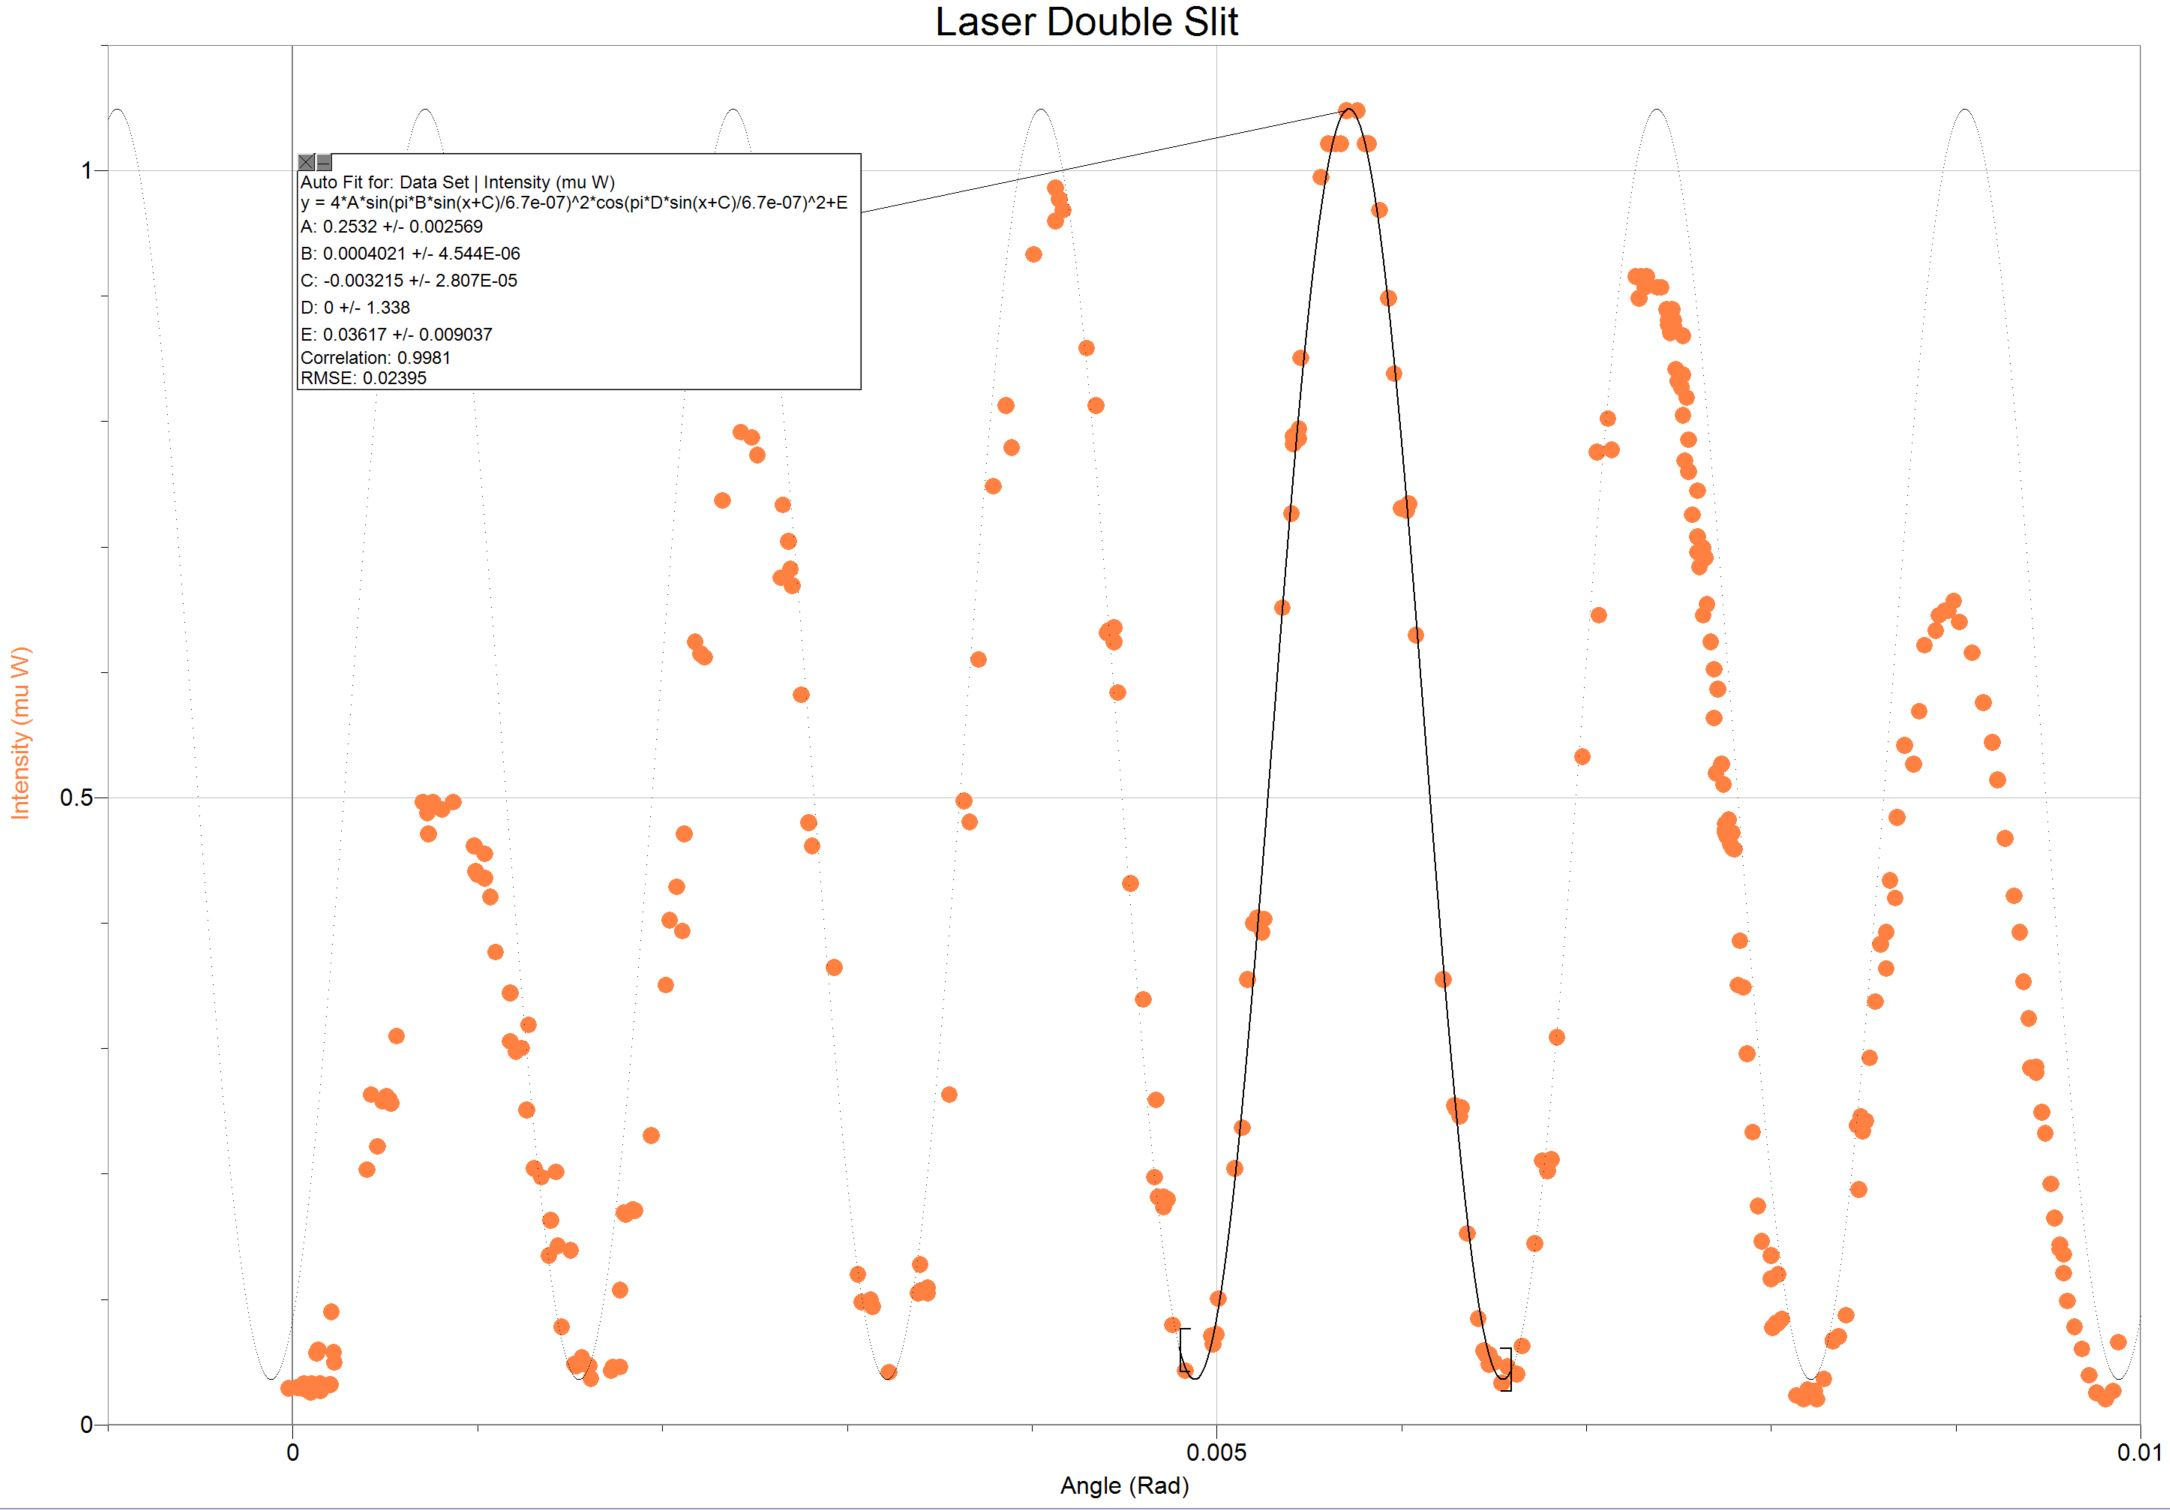
\includegraphics[height=11cm, width=15cm]{Fig1.JPG}
  
  \textbf{Figure 1, Apparent Spin-Spin Relaxation Time $(T_2^*)$}

  \vspace{10px}

  In this plot, the amplitudes is represented as a function of time. We adjust the oscilloscope to see 
  the full FID on it clearly and recorded the amplitudes as a function of time for 12 values using the cursor on the 
  screen. I used a \textbf{Linear Fit} to the logarithm of amplitudes. My experimental value of $T_2^*$, and its uncertainty 
  is $0.008663 \pm 0.0004553$ which is a smaller than $0.1 ~ ms$ as it was mentioned on the lab instructions. Also, I could use a 
  \textbf{Curve Fit} to the amplitudes to find a experimentally value for $T_2^*$.

  \vspace{10px}

  The magnetic field can be found with the help of $f_0=4.258 B_0$. We set the frequency to $15.18805 ~ MHz$, 
  therefore $B_0=3.5669 ~ KG$.  

  1) The reason this FID happens is that

  2) Why is it only an apparent spin-spin relaxation time?

  3) The physical mechanism of how the pulse sequence rotates the spins to yield the FID (Free Induction Decay)

  \pagebreak

  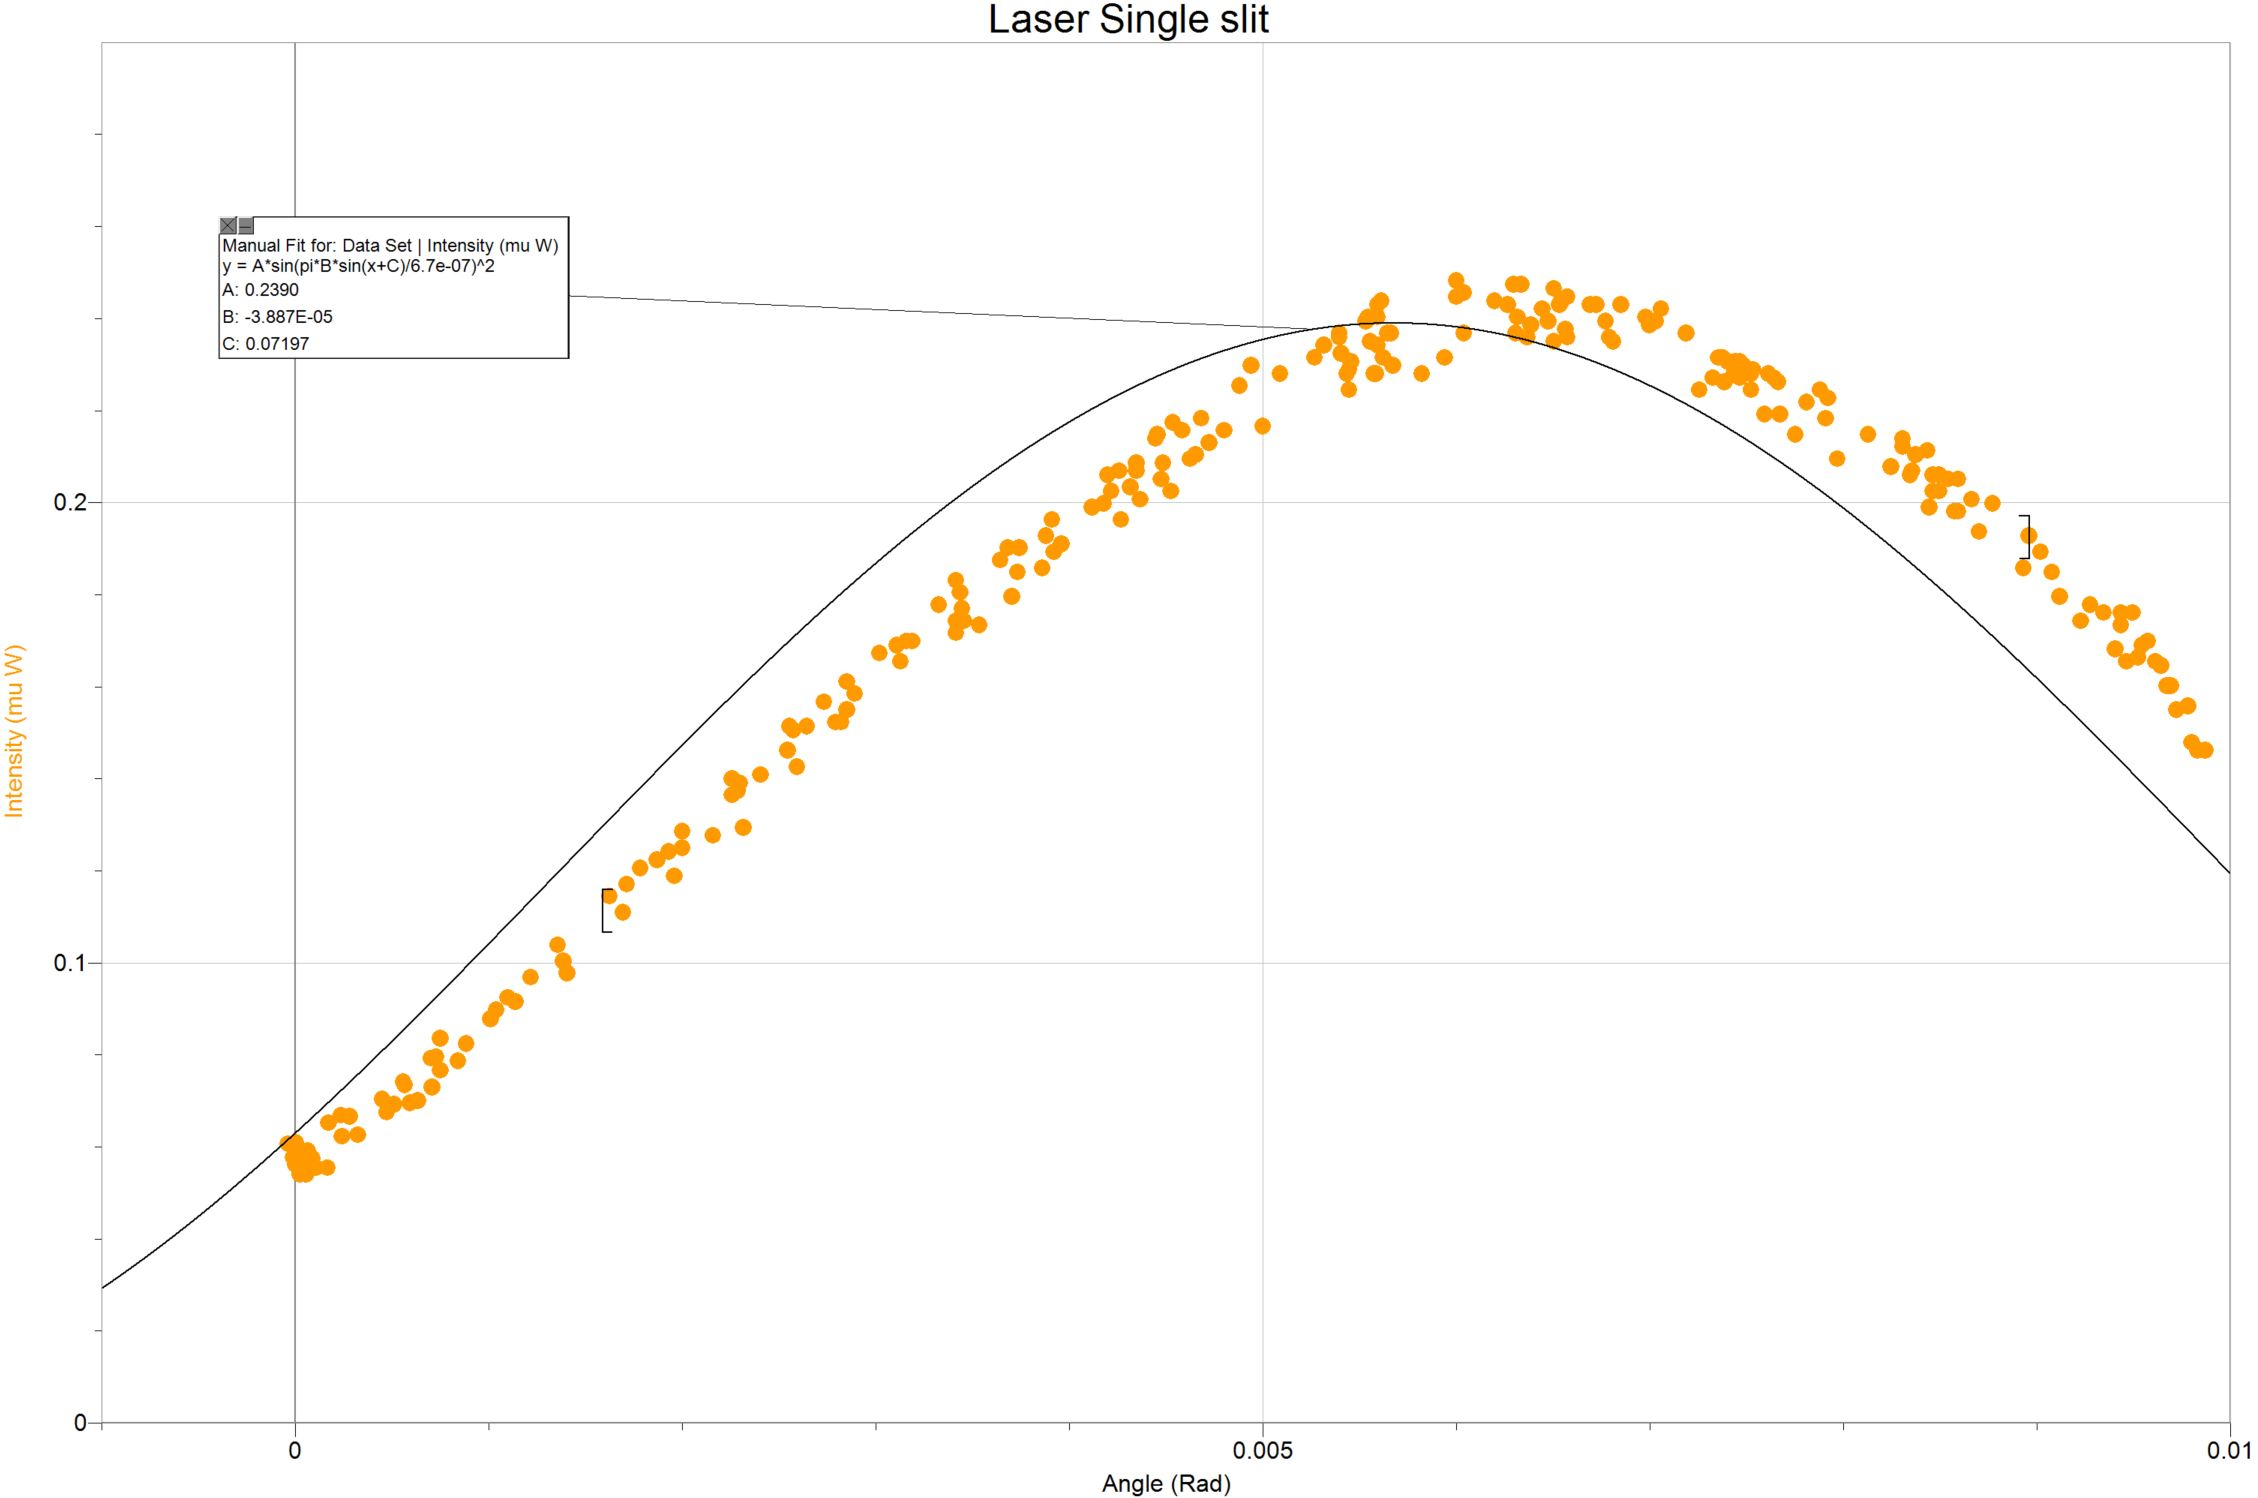
\includegraphics[height=11cm, width=15cm]{Fig2.JPG}

  \textbf{Figure 2, Spin-Lattice Relaxation Time $(T_1)$}

  \vspace{10px}

  This is the plot of the amplitude of the magnetization immediately following the B-pulse as a function of delay time. 
  I used a quadratic function to fit the data. It was found the value of $T_{min}$ as $18.88 ~ ms$ and my best 
  experimental value for $T_1$ and its uncertainty, deduced from the fit parameters for the quadratic is
  $27.2380 \pm 0.01401 ~ ms$. 
  We measured the variable \textbf{Repetition Time} by changing time scale until we saw two pulses. The time between the 
  two pusles was $7.6 \times 2= ~ 15.2 ~ ms$ which is the approximate spin-lattice relaxation time $T_1^'$. The 
  approximate spin-lattice relaxation time is consistent with my value since they are on around the same range of magnitudes.

  \pagebreak

  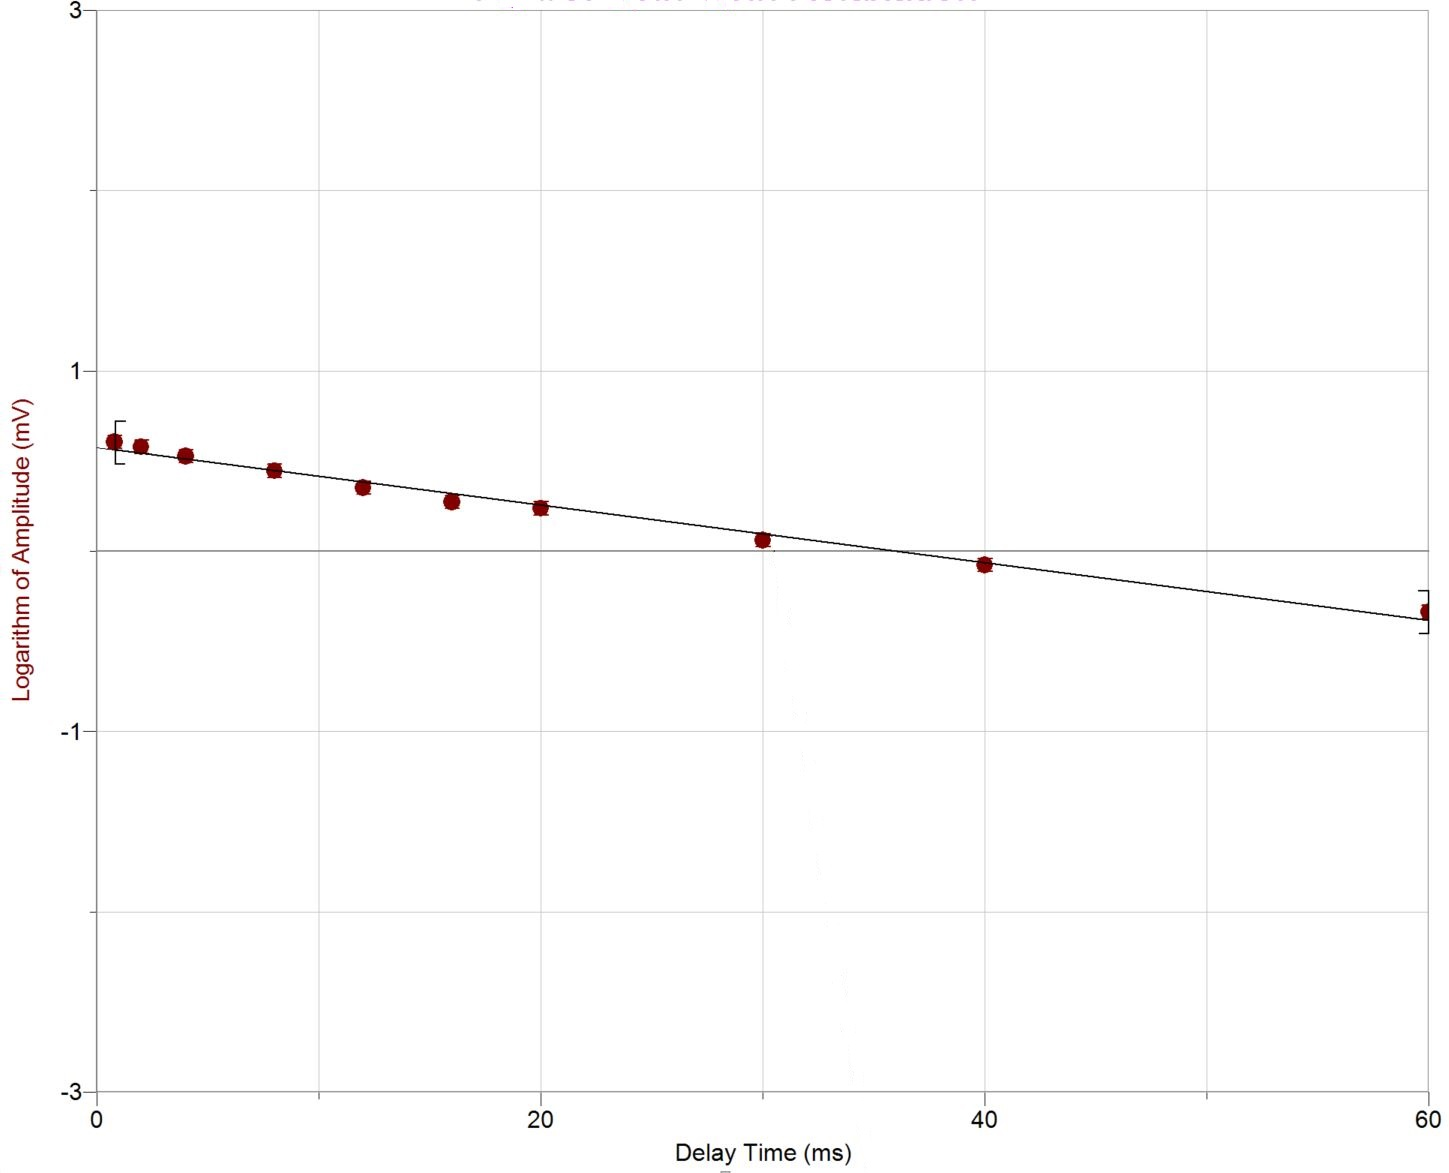
\includegraphics[height=11cm, width=15cm]{Fig3.JPG}

  \textbf{Figure 3, Spin-Spin Relaxation Time $(T2)$}

  \pagebreak


  \textbf{VI. Discussion}

  \vspace{10px}

  In this experiment...
  
  \vspace{20px}


  \textbf{VII. Conclusions}

  \vspace{10px}

  This is conclusions....
  
  \vspace{20px}


  \printbibliography

\end{document}
